
%
\begin{figure}[H]
    \centering
    \begin{subfigure}[c]{\linewidth}
        \ExampleFigure[width=\linewidth]{frame-1041}
        % 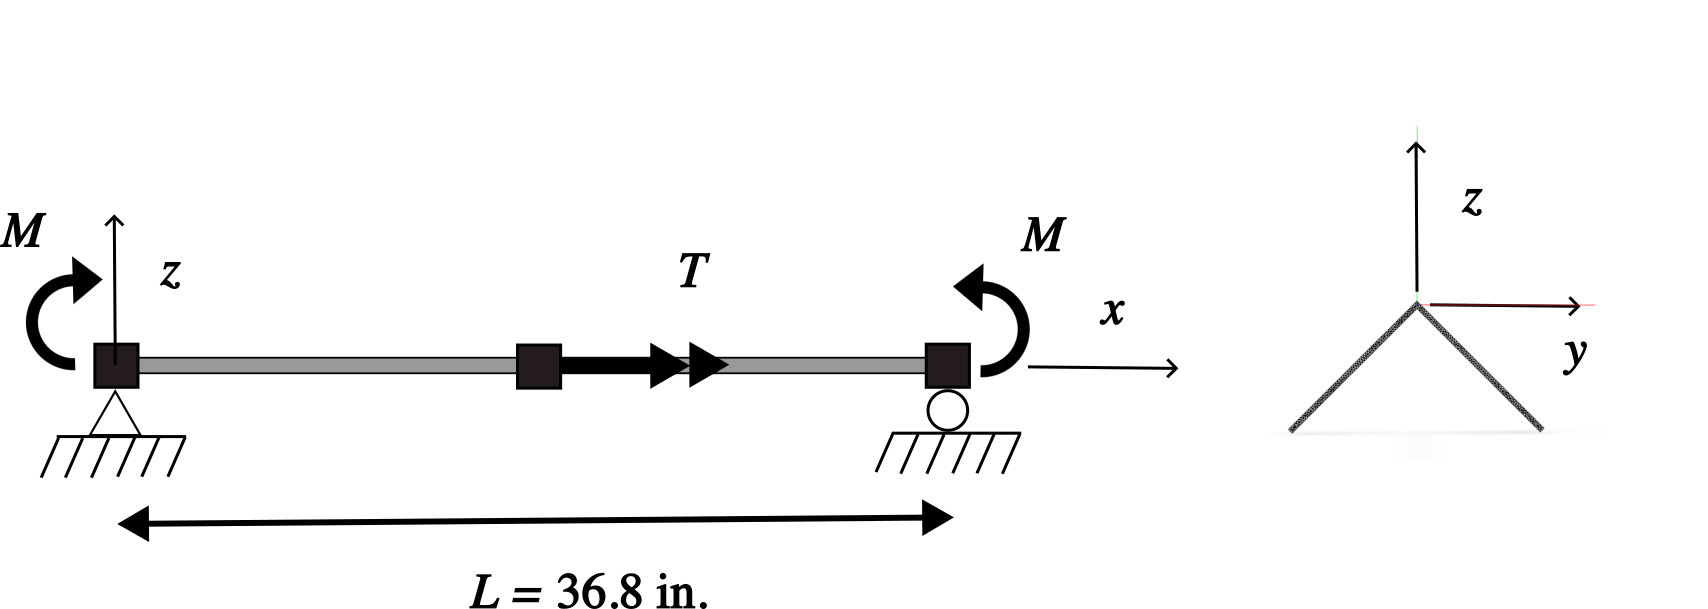
\includegraphics[width=\linewidth]{Examples/frame-1041/img/frame-1041.png}
        % \caption{Enter Caption}
    \end{subfigure}
    \caption{Model for Example~\ref{sec:frame-1041}.}
    \label{fig:frame-1041}
\end{figure}

\subparagraph{Context.}
This example reproduces an experiment by \cite{engel1953measurements} where the Wagner term \eqref{eq:wagner-gl-strain-pi} plays a central role.

\subparagraph{Setup.}
Several analyses are performed under increasing magnitudes of the applied moment \(M\), which is applied at the start of an analysis and then held constant while the torque \(T\) is gradually increased.


\FrameSection{
label/problem=frame-1041,
% Material
unit/stress={\ksi},
E=\num{10e3},
G=\num{3.75e3},
% Dimensions
unit/length={\inch},
d=1,
b=1,
t=0.03,
% Section
shape={Angle},
% kinematics/section={\eqref{eq:wagner-gl-strain-pi}},
A=\num{0.05909999999999999},
GJ={\num{1.9187014122319583e-05} $G$},
%
energetic/GAy={\num{0.4208961167529166} $GA$},
energetic/GAz={\num{0.420865659885045} $GA$},
energetic/GAyz={\num{-0.002756177128790147} $GA$},
energetic/GAzy={\num{-0.0027561771287902053} $GA$},
energetic/ShiftTwistY={\num{0.0003273069170497386}},
energetic/ShiftTwistZ={\num{-0.0003201187330745207}},
energetic/ShiftAxialY={\num{0.42046511765420164}},
energetic/ShiftAxialZ={\num{-0.41815520028172704}},
%
geometric/GAy={\num{0.4005505912001259} $GA$},
geometric/GAz={\num{0.4005265736826846} $GA$},
geometric/GAyz={\num{0.0058469924576155605} $GA$},
geometric/GAzy={\num{0.005851563943553937} $GA$},
geometric/ShiftTwistY={\num{0.0}},
geometric/ShiftTwistZ={\num{0.0}},
geometric/ShiftAxialY={\num{0.4041516701541693}},
geometric/ShiftAxialZ={\num{-0.4025695472113508}},
}

\subparagraph{Results.}
Both the \ForceFrame{} and \ExactFrame{} elements show excellent agreement.

\cite{du2021threedimensionala}

\begin{figure}[H]
    \centering
    \begin{subfigure}[c]{0.75\linewidth}
        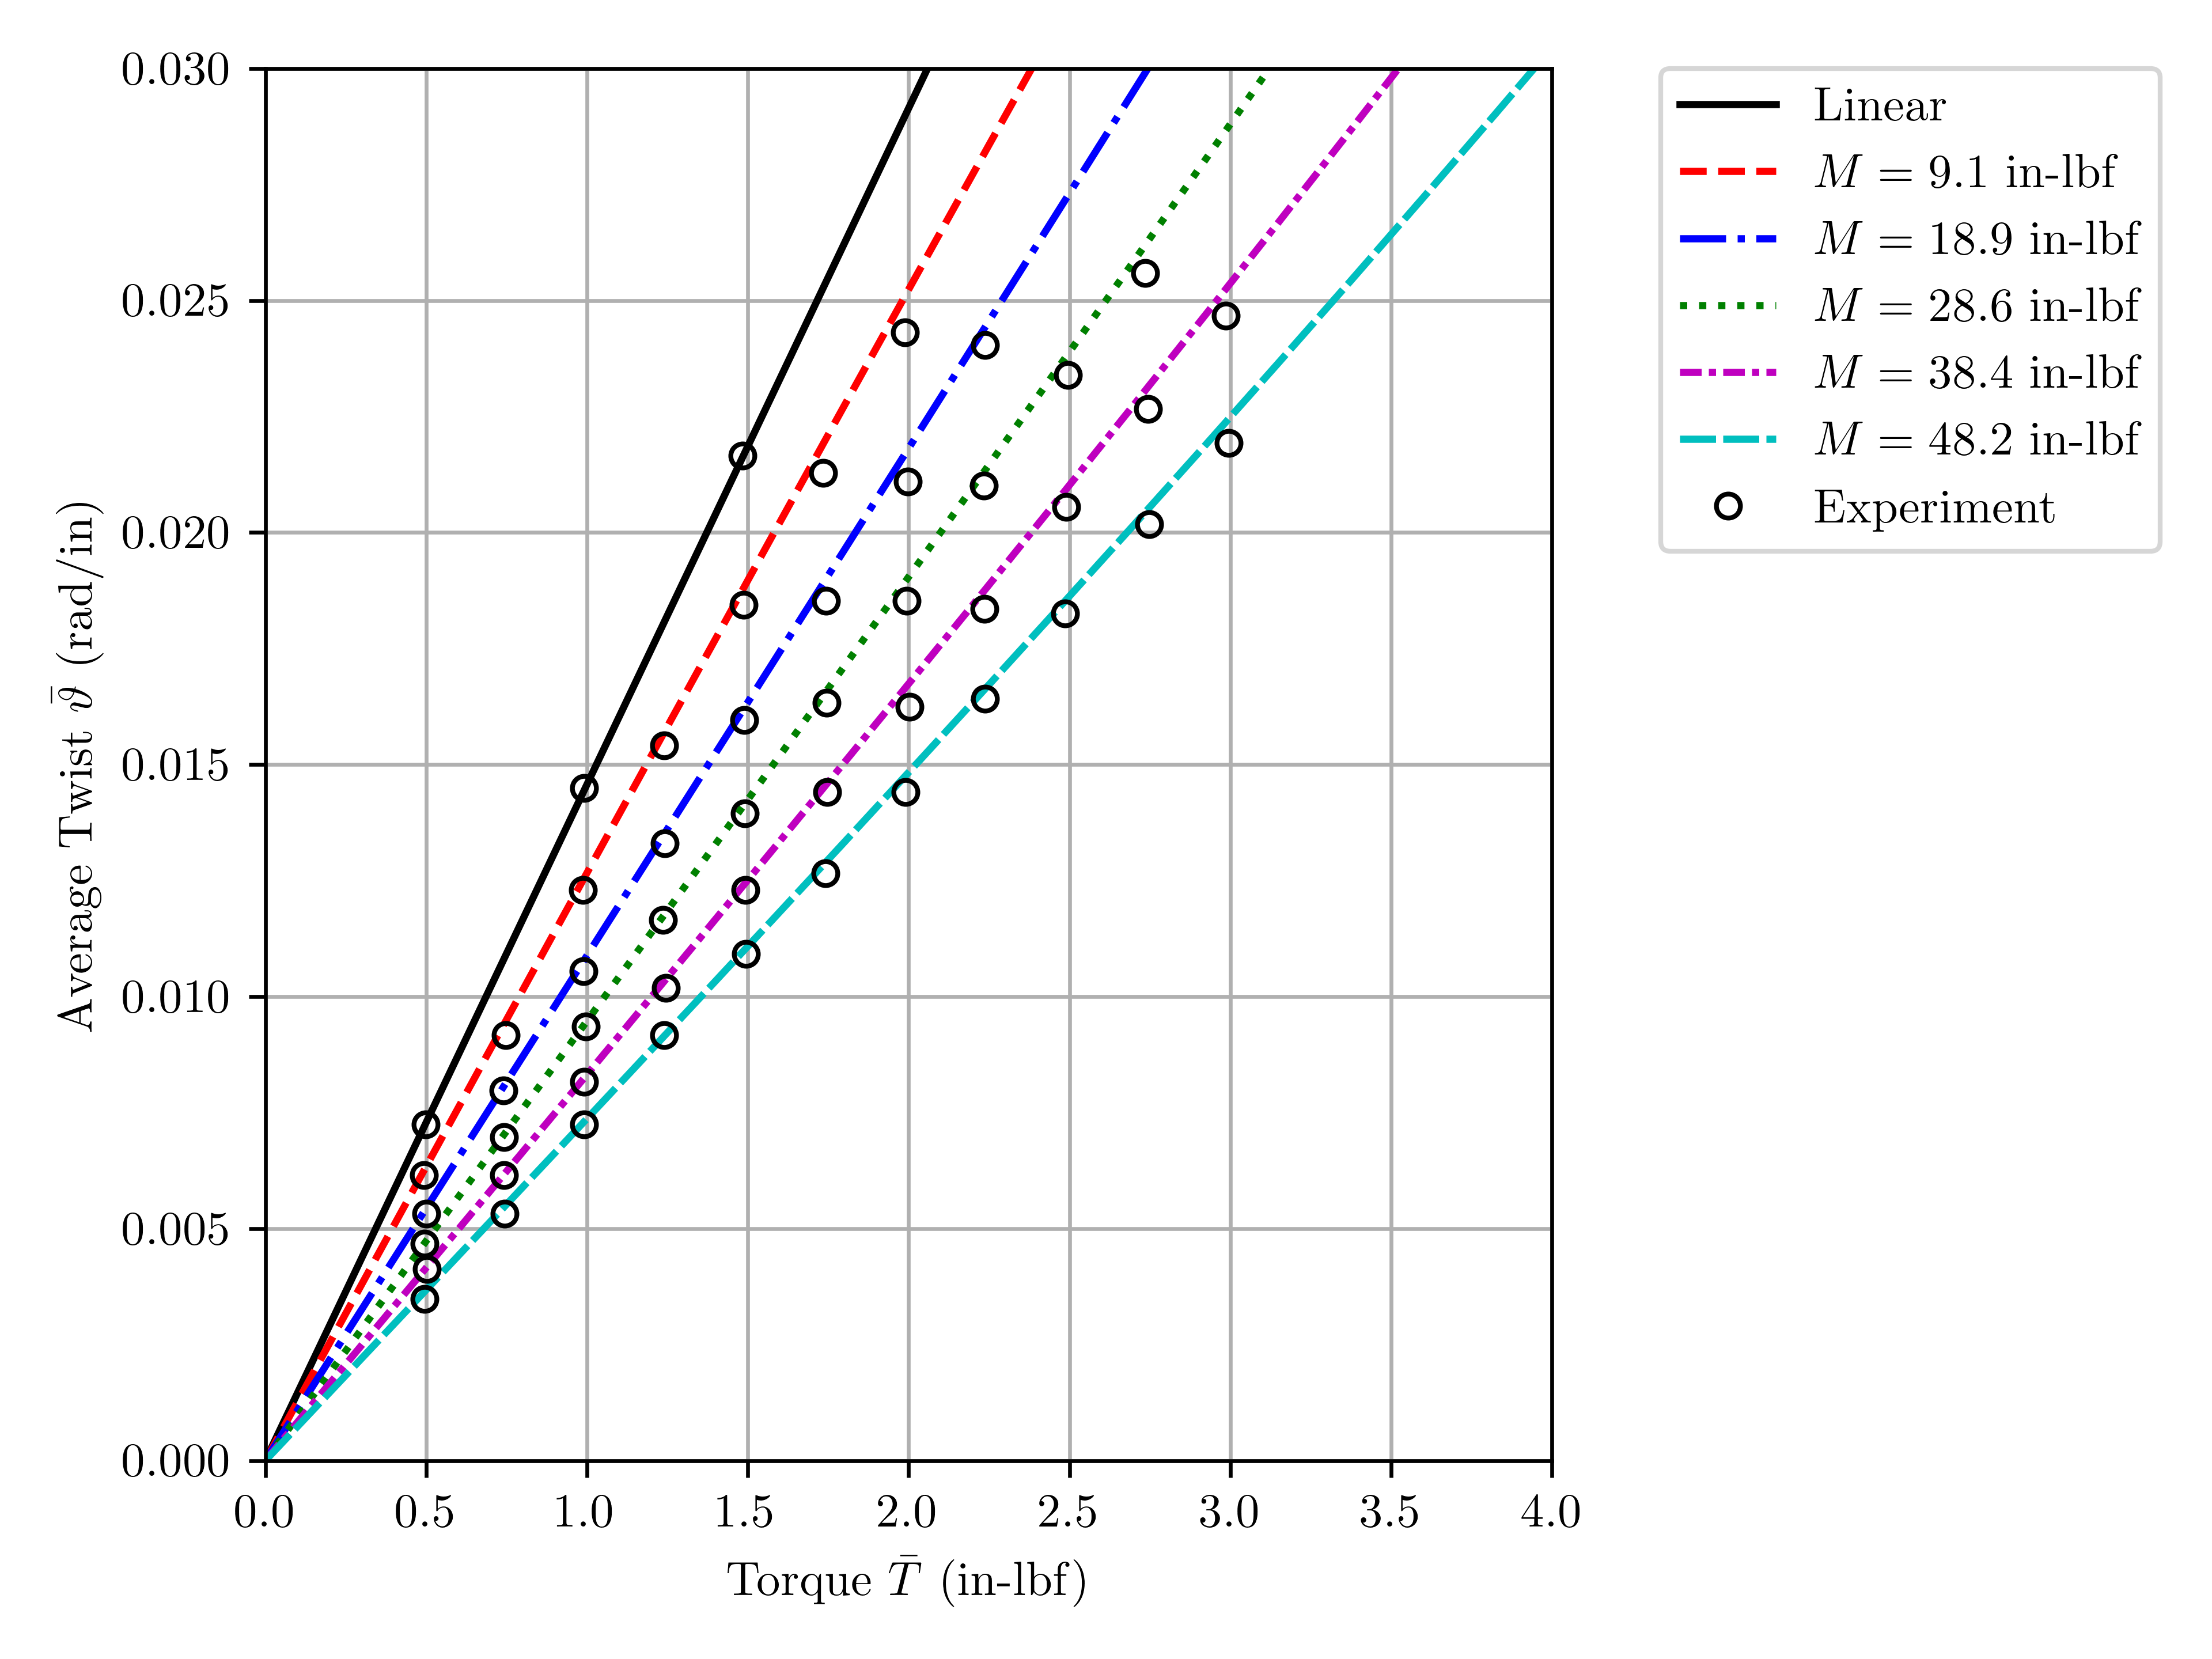
\includegraphics[width=\linewidth]{Examples/frame-1041/img/frame-1041-solution.png}
    \end{subfigure}
    \caption{Comparison with the experiment by \cite{engel1953measurements} for Example~\ref{sec:frame-1041}.}
    \label{fig:frame-1041-solution}
\end{figure}